% pain
% consider toggling word wrap in your editor
\documentclass[11pt, titlepage]{article}
\usepackage[utf8]{inputenc}
\usepackage[english]{babel}


% bibliography
\usepackage[
backend=biber,
style=numeric,
sorting=ynt
]{biblatex}
\addbibresource{refs.bib}

% useful packages
\usepackage{amsmath}
\usepackage{graphicx}
\usepackage[colorlinks=true, allcolors=blue]{hyperref}

\usepackage{listings}
\usepackage{xcolor}

% US paper
\usepackage[letterpaper, margin=1in]{geometry}
\usepackage{setspace}
\onehalfspacing

% move page number
\usepackage{fancyhdr}
\pagestyle{fancy}
\fancyfoot{}
\rfoot{\thepage}

\definecolor{codegreen}{rgb}{0,0.6,0}
\definecolor{codegray}{rgb}{0.5,0.5,0.5}
\definecolor{codepurple}{rgb}{0.58,0,0.82}
\definecolor{backcolour}{rgb}{0.95,0.95,0.92}

\lstdefinestyle{mystyle}{
    backgroundcolor=\color{backcolour},   
    commentstyle=\color{codegreen},
    keywordstyle=\color{magenta},
    numberstyle=\tiny\color{codegray},
    stringstyle=\color{codepurple},
    basicstyle=\ttfamily\footnotesize,
    breakatwhitespace=false,         
    breaklines=true,
    captionpos=b,
    keepspaces=true,
    numbers=left,
    numbersep=5pt,
    showspaces=false,
    showstringspaces=false,
    showtabs=false,
    tabsize=2
}

\lstset{style=mystyle}

\title{Simulating the Effectiveness of Physics-informed Machine Learning in Nonlinear Model Predictive Control for Robotic Manipulators}
\author{Asa Paparo}
\date{}

\begin{document}

\maketitle

\begin{abstract}

Existing methods of robotic motion planning rely on numerical optimization to generate control actions within constraints. One of the most successful methods of control has been Model Predictive Control (MPC), which continuously replans a trajectory by solving an online optimization problem. This means that for high dimension dynamical systems, the computational cost of MPC can rapidly become prohibitive. Physics Informed Neural Networks (PINNs) allow for the data driven creation and solving of high dimensional differential equations. Existing research has made progress in combining them, but lacks rigor and code optimization. In this paper, I develop an efficient NMPC implementation that relies on a PINN to plan movements. Then, I set up and integrate the controller with a state of the art simulation to demonstrate its effectiveness for a 7 DoF robotic arm. This development presents a significant advancement for fields that employ mobile robotics, such as manufacturing and search/rescue.
\end{abstract}

\section{Introduction}

Robotic manipulation is an area of high importance as global manufacturing increasingly relies on automation to accomplish tasks that would typically be done by humans. Advances in robotics and machine learning promise to be integral in the fourth industrial revolution, improving efficiency and worker safety \cite{industry_4.0}. Specifically, the advancement and effectiveness of industrial robotic systems is central to a developed nation's prosperity and economy. Due to high domestic costs and restrictions, offshore manufacturing is utilized by companies seeking to minimize cost of production. To improve economic conditions without worsening worker conditions, the United States must rely on robotic manufacturing \cite{manufacturing_prosperity}. Additionally, search and rescue presents a major opportunity for robotics to improve by making it safer and more efficient \cite{search_rescue}. For medicine, surgical robots can accomplish tasks with more precision and safety than their human counterparts \cite{surgical_robots}.

A primary goal of the field of control theory is the efficient and constrained control of complex dynamical systems. A highly popular approach for this is Model Predictive Control, which relies on continuously replanning a trajectory over a specific horizon \cite{mpc_industry}. In situations where high processing power is available, such as on Boston Dyanmics' robots, this is a necessary tradeoff for the flexibility of nonlinear MPC \cite{spot}. However, despite significant development on improving this controller, nonlinear MPC still suffers from requiring "enourmous computational effort" \cite{mpc_computation}. To address this, several groups have successfully used physics-informed machine learning for optimization in MPC instead of traditional methods \cite{pinn_mpc_manipulators, pinns_mpc}. A natural application of this is in control of high dimensionality robotic arms, which is made significantly more efficient by the neural network. These papers provide evidence in favor of PINN-based MPCs for controlling lower dimensional systems, so I hope to use a robotics code framework called Drake \cite{drake} to simulate the control of a high dimensional industrial arm.


    % Current methods of robotic manipulation rely on predefined systems and control algorithms to function effectively. \cite{underactuated} This is a effective in most scenarios. However, it requires retuning for any change to the system. In consumer or high risk situations, it may be impractical to retune systems periodically to account for changes to the physical hardware. In this paper, I propose an alternative paradigm using physics-informed machine learning to correct for changes to the system on the fly.

    % The goal of this experiment is to examine the effectiveness <develop a new generation> of PINN (Physics Informed Neural Networks) in adapting the model of a system on the fly. This would enable the dynamic updating of control algorithms, given little prior knowledge about external conditions. For example, a manipulator should be able to grasp any arbitrary load and continue to plan trajectories effectively. In order to test this, I derive the governing equations of motion for a simple 2-DOF arm system and use drake \cite{drake} to run discrete simulations of MPC and trajectory planning for this arm. To verify my hypothesis, I modify the load attatched to the manipulator midway through the simulation and record the new effectiveness of controlling it.


    % Robotic manipulation is an area of high importance as global manufacturing increasingly relies on automation to accomplish tasks that would typically be done by humans. Advances in machine learning promise to be as impactful as an industrial revolution, with potential to deliver widespread benefits to civilization.\cite{ai_on_industrial} Specifically, advances in robotic automation for manufacturing and medicine have potential to reshape their industries for the better. In the case of manufacturing, this allows for significantly greater productivity and worker safety. For medicine, surgical robots can accomplish tasks with more precision and safety than their human counterparts. \cite{2, 3, 4, 5} Automation in manufacturing is also critical for the prosperity and improvement of our modern society. For example, relevance in the global economy is viewed as core to American national security, and automation is an essential part in that \cite{6}. Such importance is further exacerbated by declining birth rates in industrialized nations, which means a smaller workforce to support a growing aging population \cite{tandf2}. Because of this, advances in robotic automation are essential in overcoming global challenges and improving the standard of living around the world.
    
    % Robotic trajectory optimization is a well known field, however, implementations often suffer from relatively long compute times for numerical optimization. Additionally, successful throwing implementations for rigid robotic arms exist. However, they all 


    % analytical dynamics


\section{Methods}

\subsection{Nonlinear Model Predictive Control (NMPC)}

\begin{figure}[hbt!]
\centering
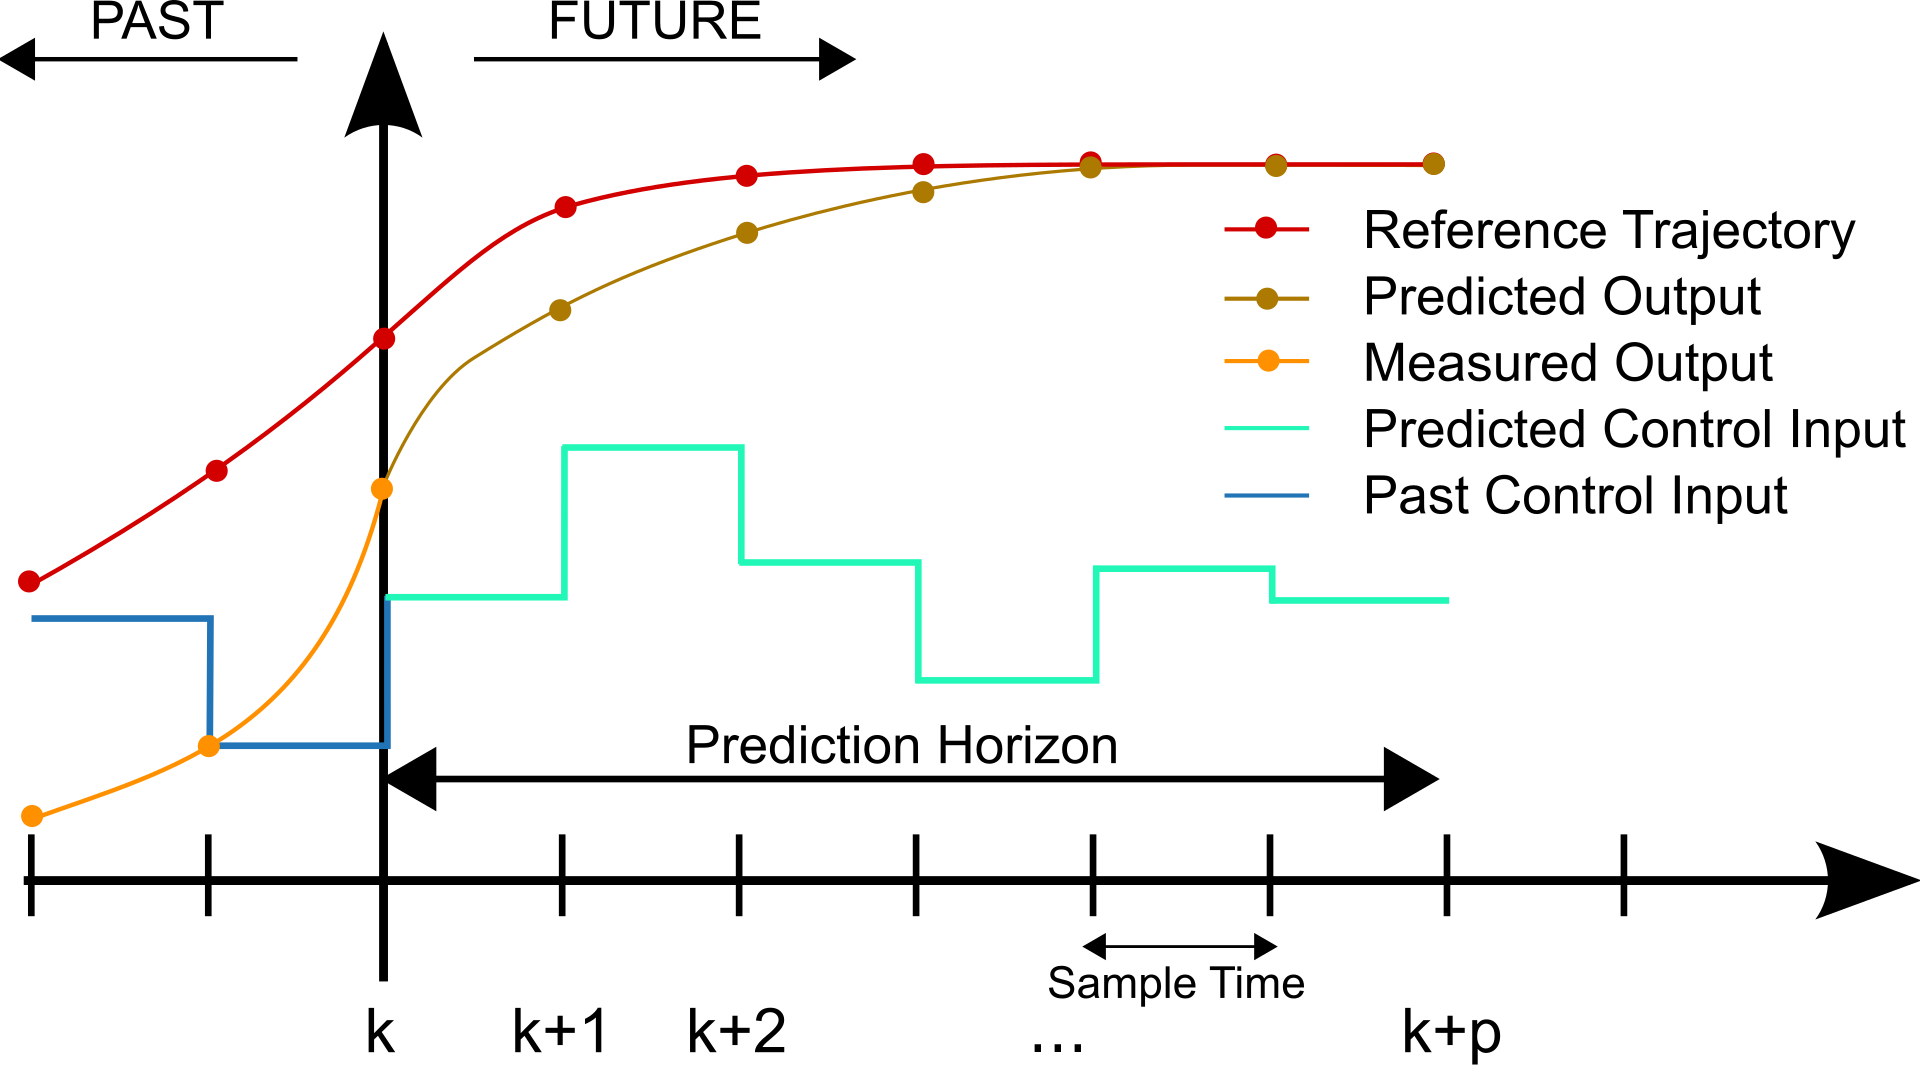
\includegraphics[width=0.5\linewidth]{MPC_scheme_basic.png}
\caption{\label{fig:mpc}A diagram of model predictive control by Martin Behrendt \cite{mpc_diagram}. It shows the planning of a new trajectory over time in comparison to the previously planned trajectory. }
\end{figure}

Model predictive control \cite{MPC} and its nonlinear variation are an algorithm with several steps.
\begin{enumerate}
    \item Create an optimized trajectory from current to target states over the specified horizon
    \item Follow the first discrete state within the larger trajectory
    \item Repeat with the new state
\end{enumerate}

The trajectory calculated at each step is based on an optimal control law, which minimizes a cost function $J(x, u)$ \cite{Illinois_motion}.

\begin{equation}
J(x,u) = \int_0^\infty L(x(t),u(t),t) dt.
\label{eq:CostFunctional}
\end{equation}

\begin{equation}
\begin{gathered}
x^\star, u^\star = \arg \min_{x,u} J(x,u) \\
\dot{x}(t) = f(x(t),u(t)), \forall t \\
x(0) = x_0
\end{gathered}
\label{eq:OptimalControl}
\end{equation}

This would be solved by a PINN trained to the dynamics of the system, however, I was unable to successfully implement this on a deadline. For the remainder of this project, I use an "InverseDynamicsController," which uses the system's dynamics to convert PID control output into applicable voltages.

\subsection{Simulation}

To create an effective simulation for the system, I use Drake. The specific system I control is a 7 degrees of freedom KUKA iiwa arm, with documentation from MIT Manipulation \cite{manipulation}. Since I could not immediately get a PINN working

\begin{figure}[hbt!]
\centering
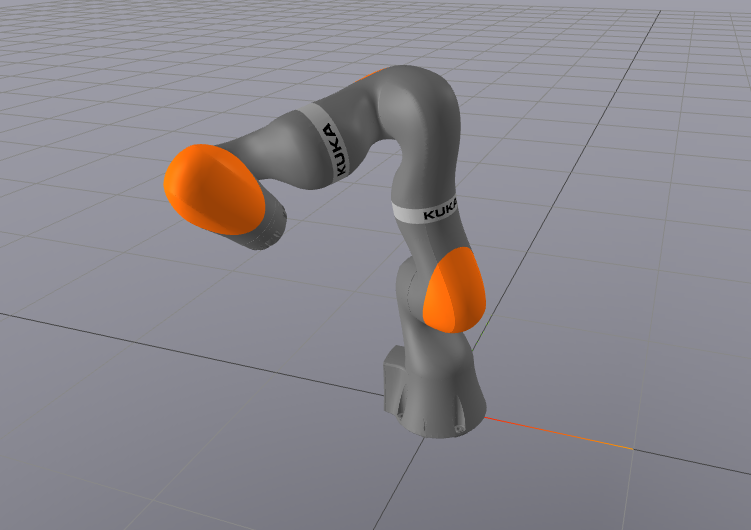
\includegraphics[width=0.25\linewidth]{iiwa.png}
\caption{\label{fig:iiwa}A visualization of the simulation, using Meshcat and the iiwa14 urdf file.}
\end{figure}

\begin{lstlisting}[language=Python]
meshcat = StartMeshcat()
builder = DiagramBuilder()

# Adds both MultibodyPlant and the SceneGraph, and wires them together.
plant, scene_graph = AddMultibodyPlantSceneGraph(builder, time_step=1e-4)
# Note that we parse into both the plant and the scene_graph here.
iiwa_model = Parser(plant, scene_graph).AddModelsFromUrl("urdf url here")[0]
plant.WeldFrames(plant.world_frame(), plant.GetFrameByName("iiwa_link_0"))
plant.Finalize()

# Set up visualizer
visualizer = MeshcatVisualizer.AddToBuilder(builder, scene_graph, meshcat)

# PID controller
n = plant.num_positions()
kp = [100] * n
ki = [1] * n
kd = [20] * n
iiwa_controller = builder.AddSystem(
    InverseDynamicsController(plant, kp, ki, kd, False)
)
iiwa_controller.set_name("iiwa_controller")

# Wire simulation
builder.Connect(
    plant.get_state_output_port(iiwa_model),
    iiwa_controller.get_input_port_estimated_state()
)
builder.Connect(
    iiwa_controller.get_output_port_control(),
    plant.get_actuation_input_port()
)
diagram = builder.Build()
diagram.set_name("iiwa diagram")

context = diagram.CreateDefaultContext()
plant_context = plant.GetMyMutableContextFromRoot(context)

# Arbitrary starting config
q0 = np.array([-1.5, 0.1, 0, -1.2, 0, 1.6, 2])
w0 = 2 * q0
x0 = np.hstack((q0, w0))
plant.SetPositions(plant_context, q0)
iiwa_controller.GetInputPort("desired_state").FixValue(
    iiwa_controller.GetMyMutableContextFromRoot(context), x0
)

# Simulator
simulator = Simulator(diagram, context)
simulator.set_target_realtime_rate(1.0)

meshcat.StartRecording()
simulator.AdvanceTo(10.0)
meshcat.StopRecording()
meshcat.PublishRecording()

\end{lstlisting}

This code sets up a simulation, with a structure shown in figure \ref{fig:diagram}. Notably,

\section{Results}

\begin{figure}[hbt!]
\centering
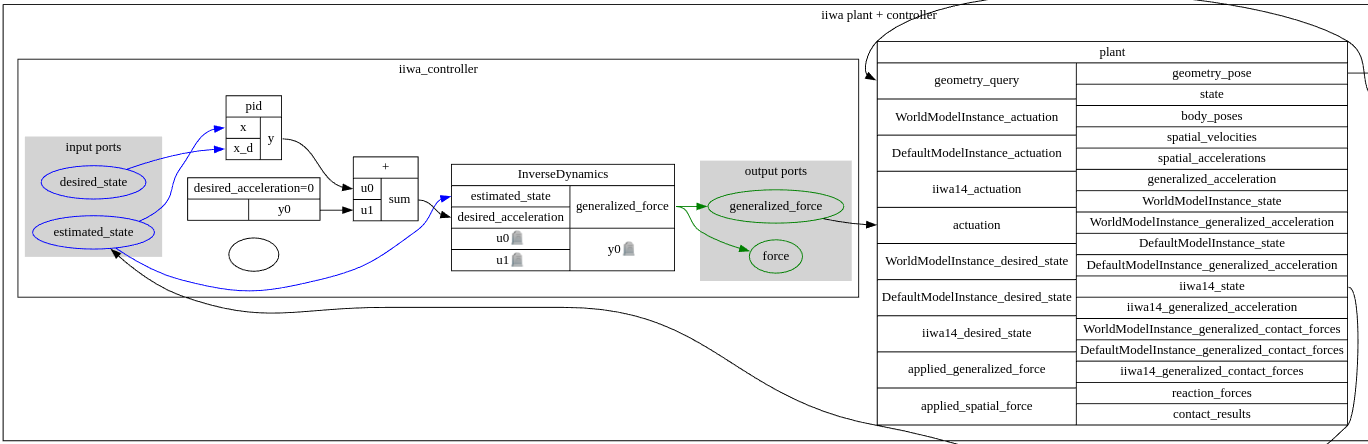
\includegraphics[width=1\linewidth]{diagram.png}
\caption{\label{fig:diagram}A flow input/output diagram of a PID controller connected to the iiwa system, generated by Drake.}
\end{figure}

\begin{figure}[hbt!]
\centering
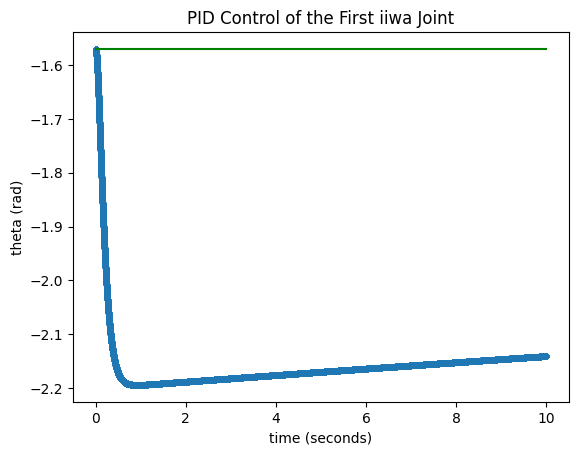
\includegraphics[width=0.5\linewidth]{pid.png}
\caption{\label{fig:pid}A graph of the base joint of the iiwa arm under inversion PID control. As you can see, because the arm is fully actuated, the position very quickly approaches its setpoint.}
\end{figure}

For this project, while I was able to make progress with the simulation and nonlinear model predictive controller, I was unable to successfully finish a python implementation of the neural network on time. This limited my ability to collect data on every component working as a whole. However, as shown in figure \ref{fig:diagram}, I was successful in creating the closed loop control simulation based on the loaded arm dynamics. Overall, the tools I employed for the simulation of this robot were very effective, and will likely see significantly more prevalence going forward. Lastly, as shown in \ref{fig:pid}, I demonstrated the effectiveness of seperate PID control for individual components of the arm.

\section{Discussion}

My results are rather inconclusive regarding the effectiveness of PINN-based NMPC, however they convey the utility of simulation in the robotics field. It is important to note, that for these controllers to reach widespread adoption, a well documented and high performance implementation will have to exist, considering the technical barrier to implementing it from scratch.

\printbibliography

\end{document}
